\chapter{Cjevovod}
\label{chap:cjevovod}

Cjevovod je arhitektonski programski obrazac u kojem podaci prolaze kroz filtre
koji su postavljeni jedan za drugim. Time se simulira jedan tok koji iz ulaznih
podataka transformacijom kroz filtre generira izlazne podatke. U ovome projektu
cjevovodna arhitektura je samo logički kostur koji se enkapsulira unutar razreda
\emph{Pipeline}. Iako je u začetku razvoja aplikacije svaki filter bio zaseban
proces, vrlo ubrzo je ustanovljeno kako većina filtera generira podatke koji su
potrebni na raznim mjestima u cijeloj aplikaciji te se činilo lakše imati sve
podatke u memoriji pojedinog cjevovoda. To je omogućilo da razred
\emph{Pipeline} naslijedi razred \emph{Thread} iz modula \emph{threading} te se
može pozivati kao zasebna dretva.

Tok cjevovoda se može vidjeti na slici \ref{fig:cjevovod}. Ulaz u cjevovod
predstavljaju paralogni proteini u FASTA formatu koje zadaje korisnik. Ti se
podaci zadaju pri stvaranju objekta \emph{Pipeline} kako bi se mogli zapisati na
disk u direktorij vezan za instancu \emph{Pipeline-a}. Stvarni objekt kojeg
prima konstruktor \emph{Pipeline-a} je rječnik prilagođen uporabi mrežna
aplikacije, što je detaljnije opisano u poglavlju \ref{chap:server}.

\begin{figure}[h!]
\centering
%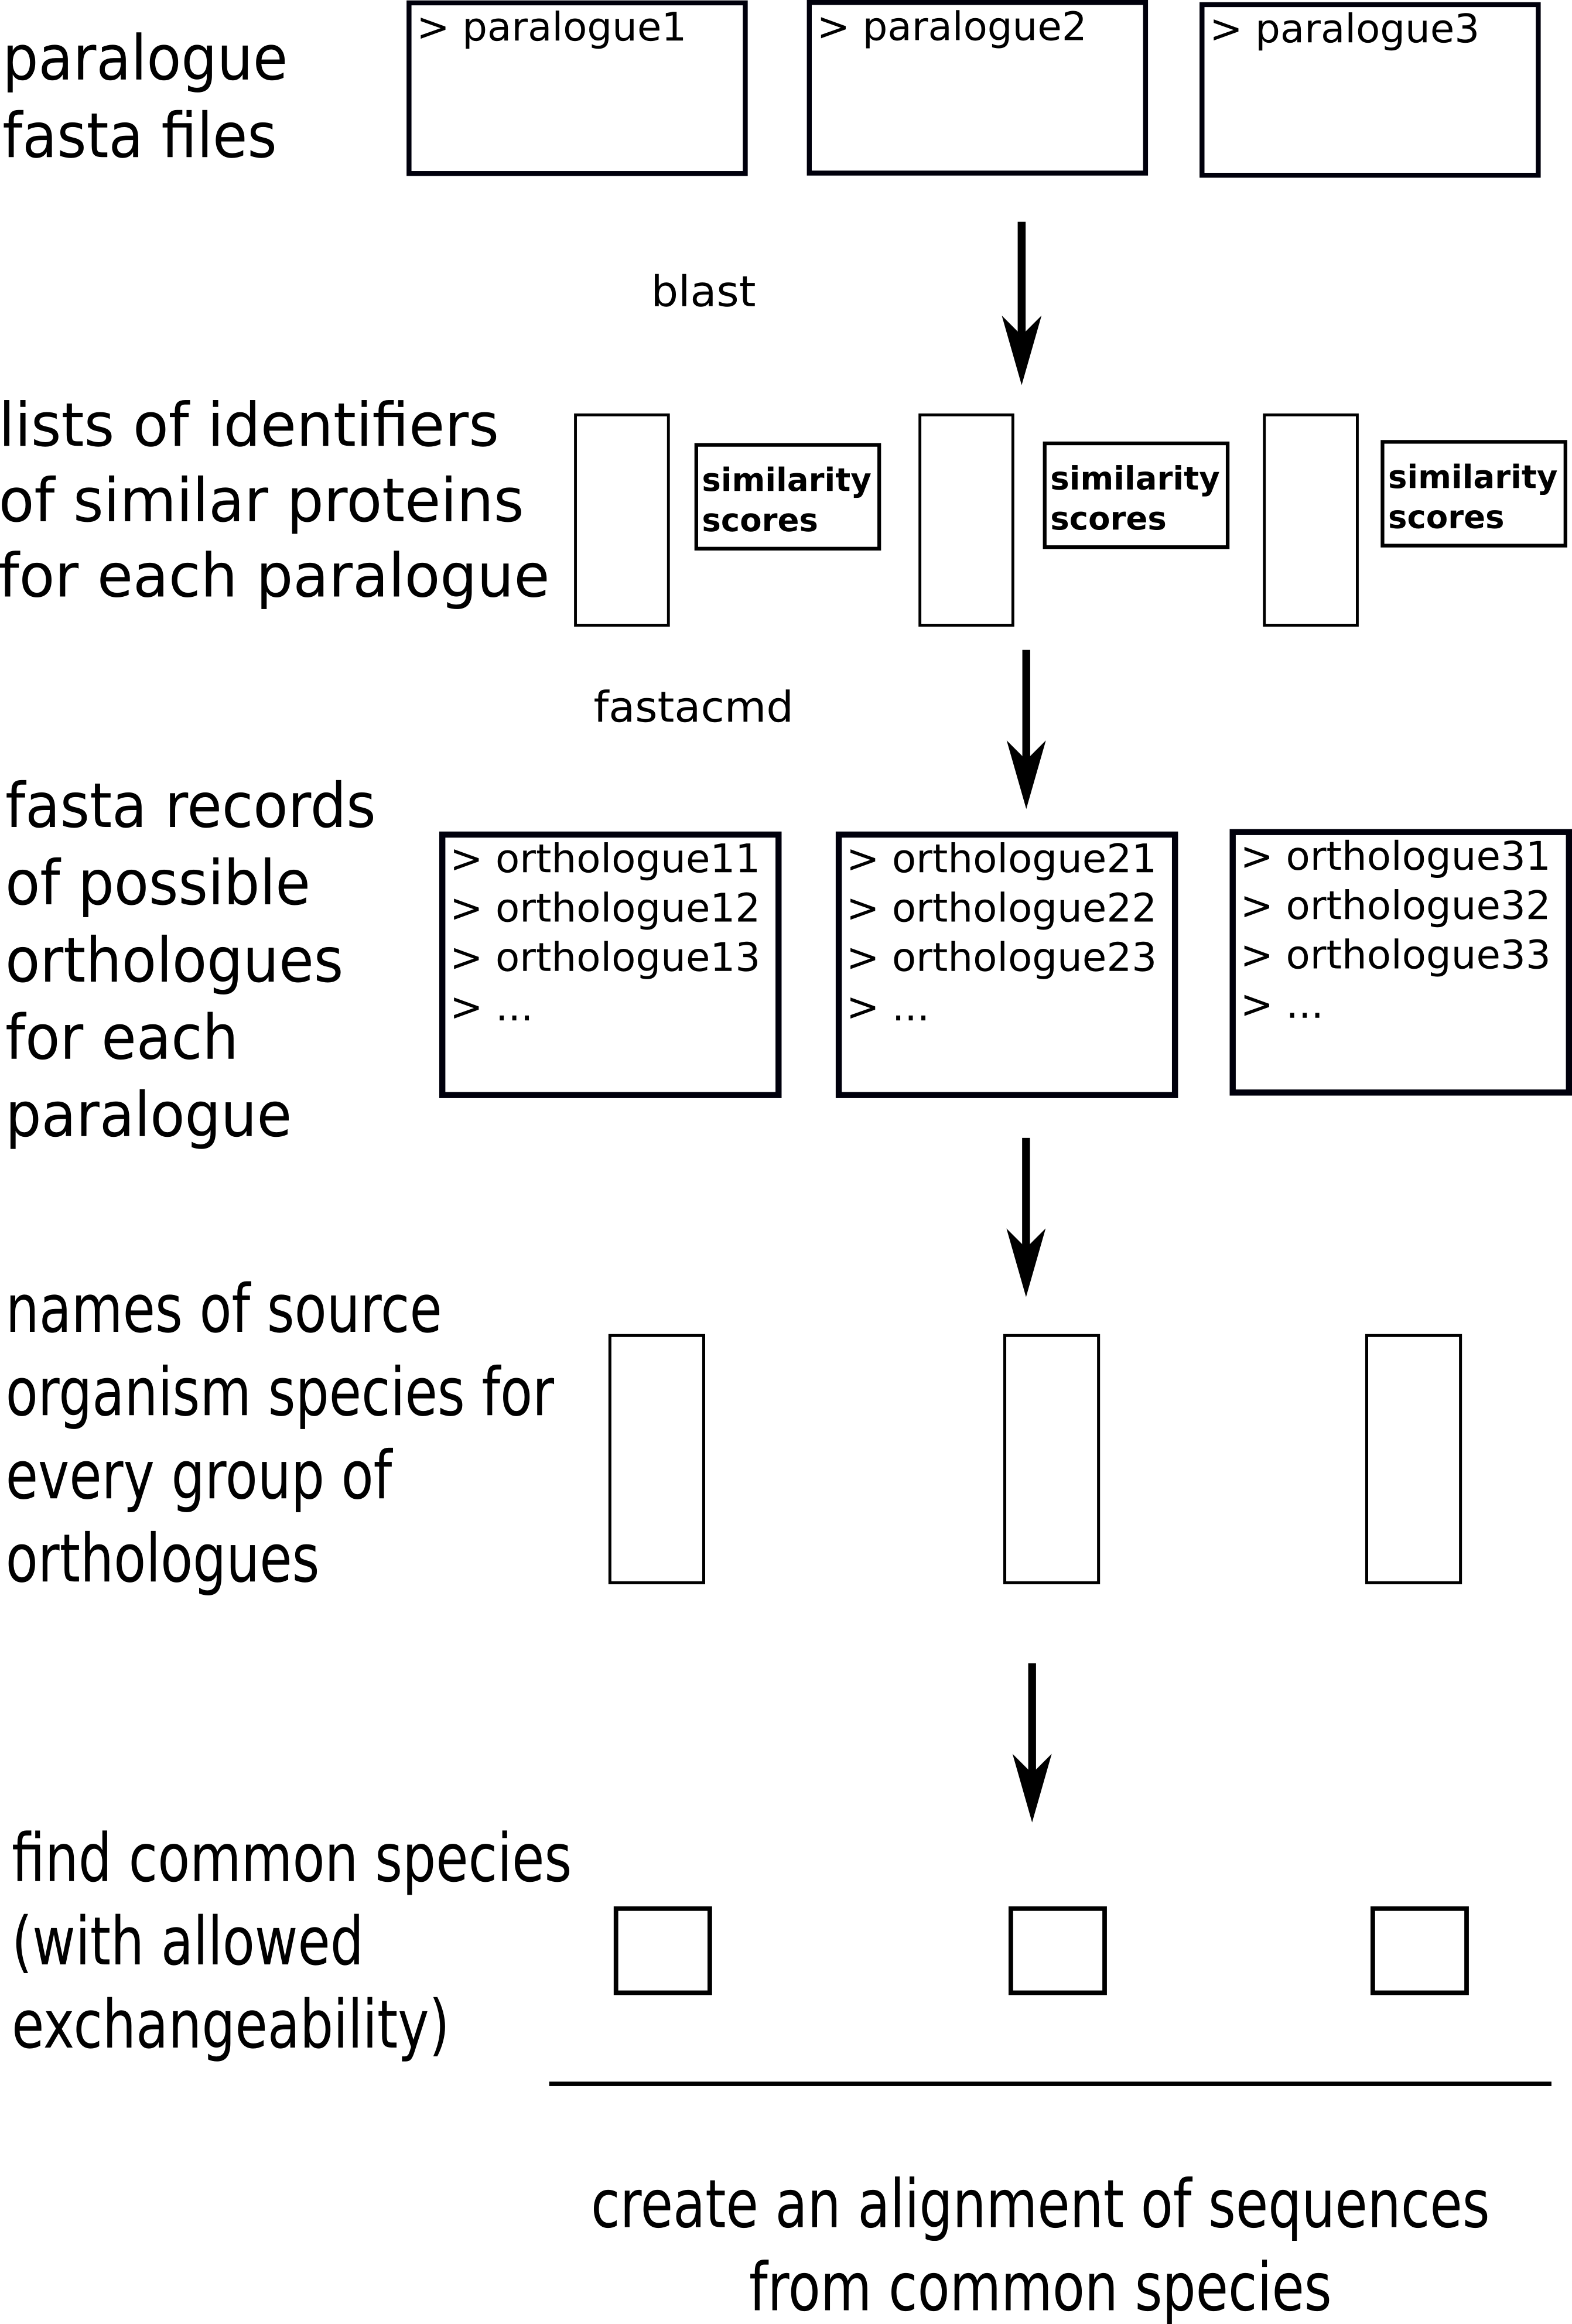
\includegraphics[width=1.0\linewidth]{figures/cjevovod.png}
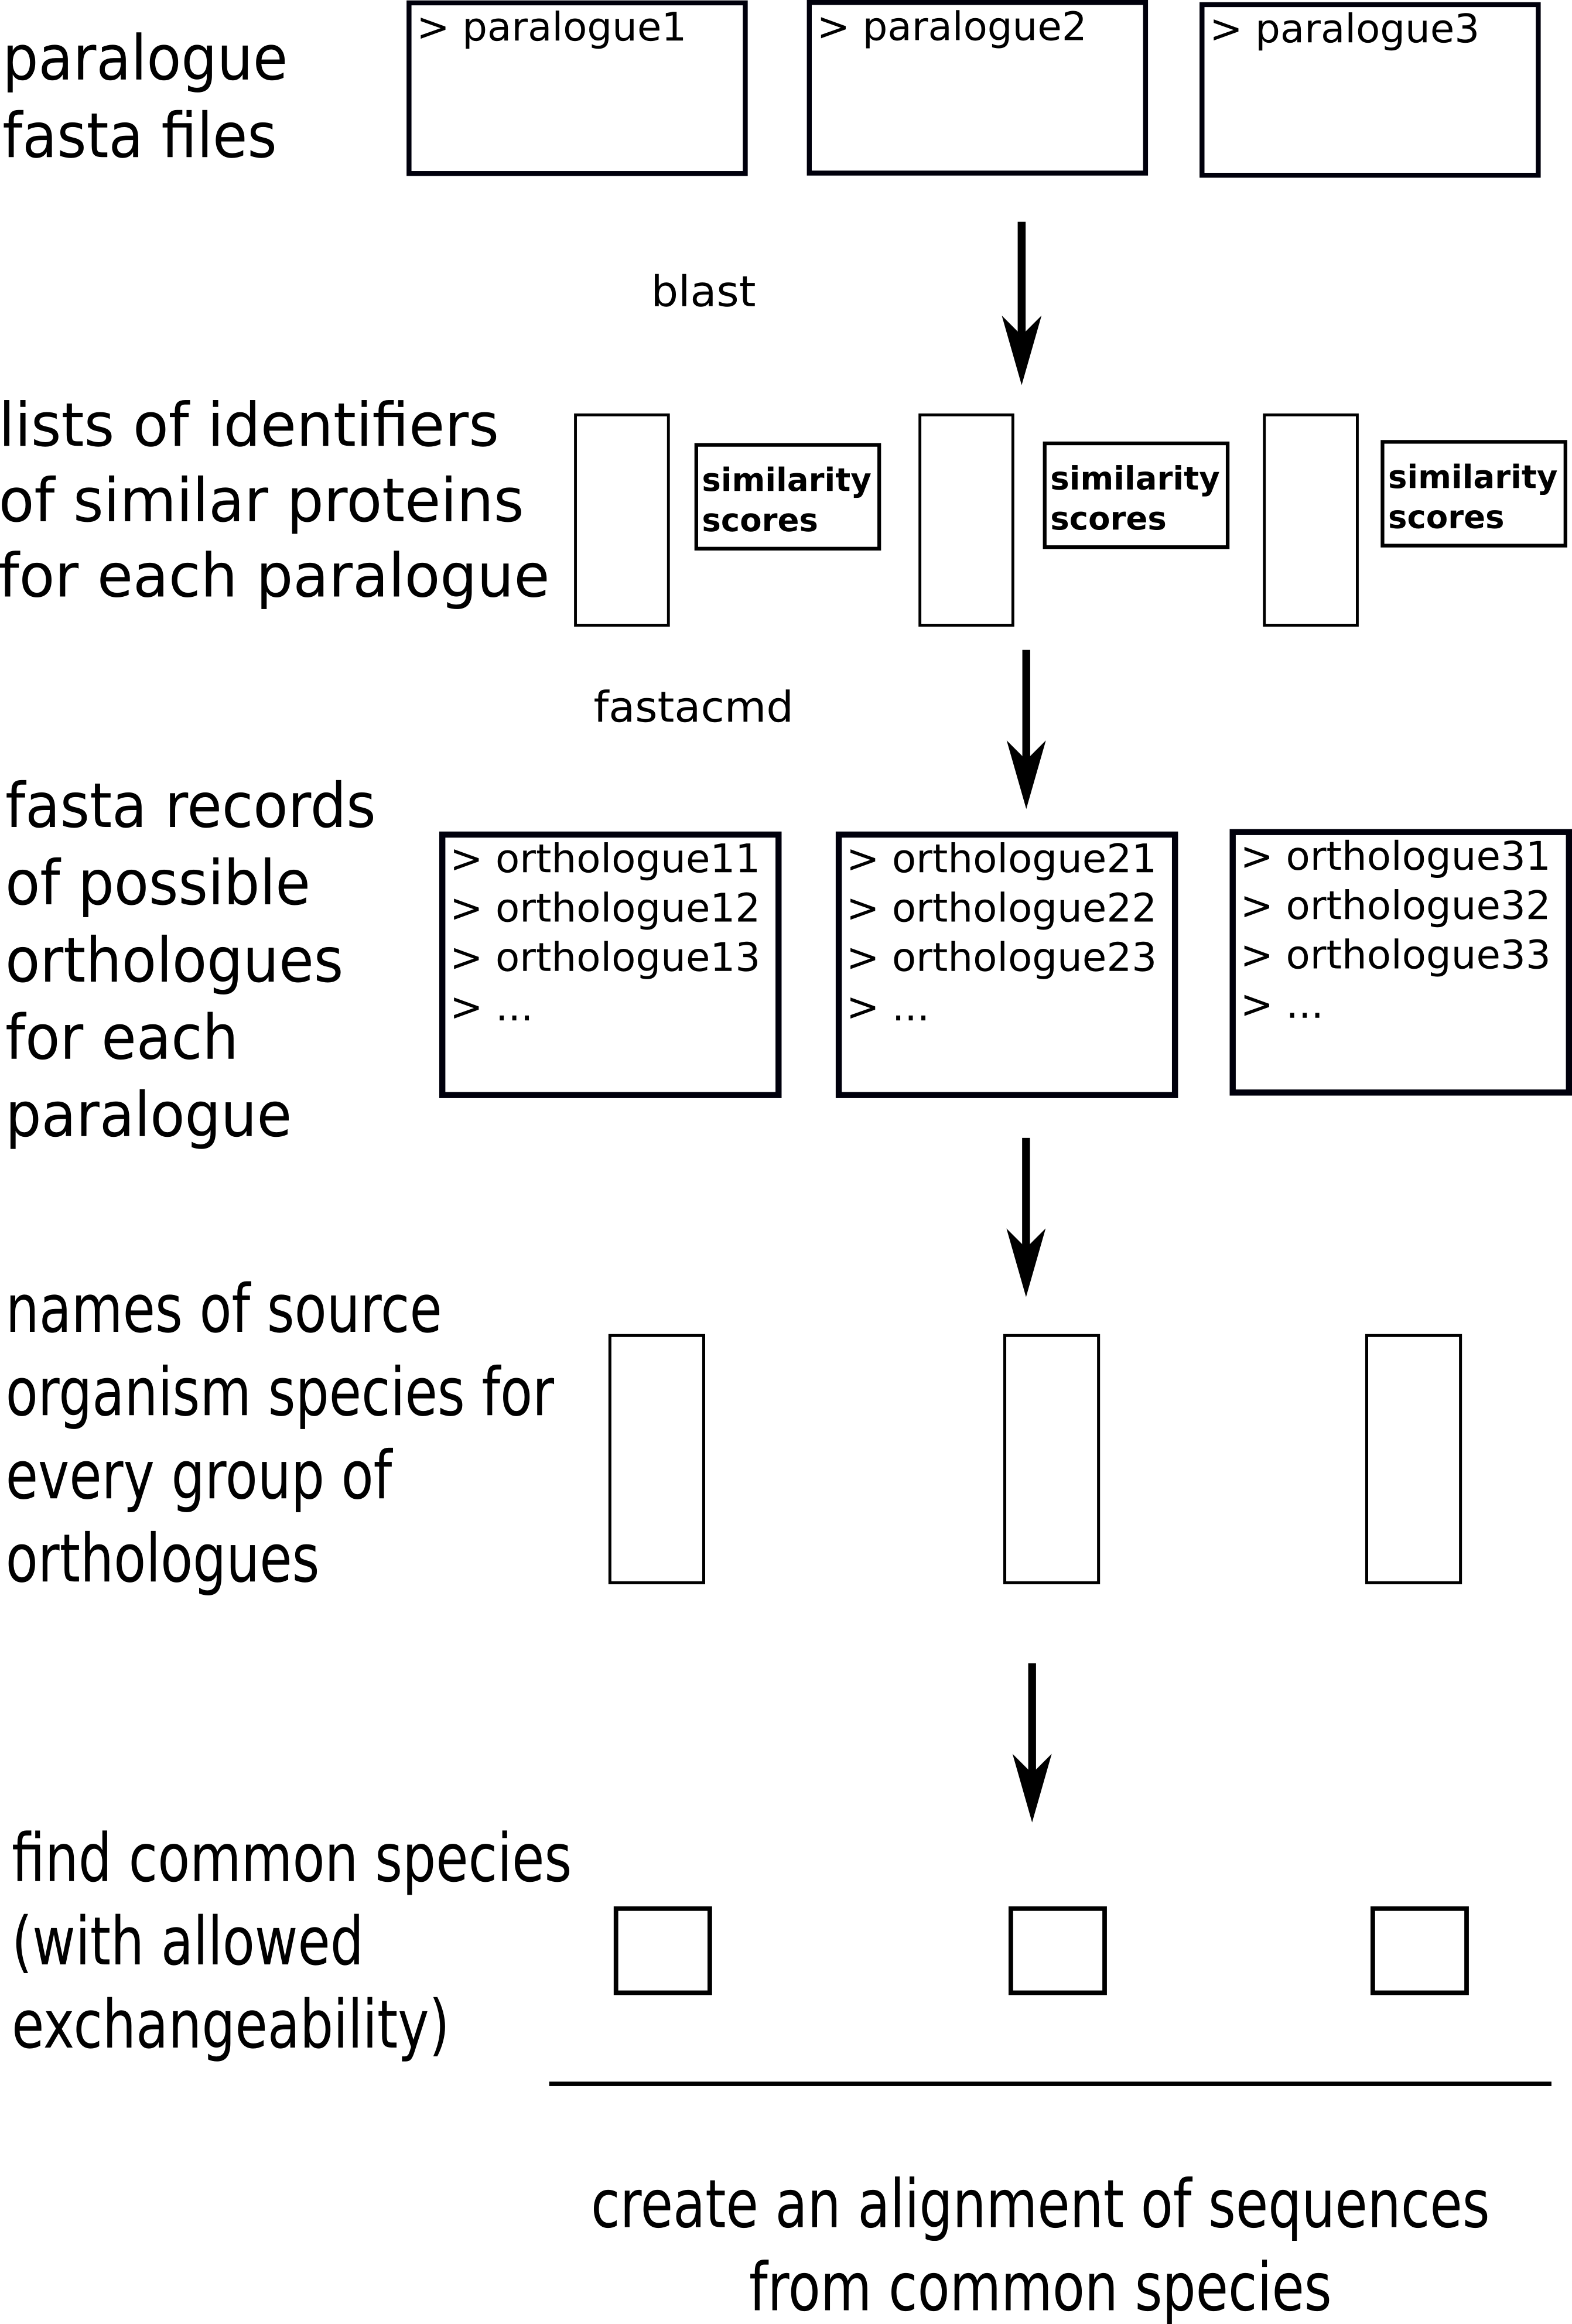
\includegraphics[width=4.5in]{figures/cjevovod.png}
\caption{Protok podataka kroz cjevovod. Radije se prikazuju podaci nego filtri
zbog boljeg uvida u rad cjevovoda}
\label{fig:cjevovod}
\end{figure}

Pri pokretanju cjevovoda za svaku se od unesenih sekvenci stvara objekt razreda
\emph{ProteinHolder} prilikom čega se obavljaju pozivi filtara nezavisnih za
svaku pojedinu sekvencu. Prvi filter koji se koristi je alat
\emph{BLAST}\cite{altschul1997gapped} te je izveden kao poziv zasebnog izvršnog
programa \emph{blastall} na sljedeći način:

\begin{lstlisting}[language=bash]
blastall -p blastp -i <ulaz-FASTA> -d <nr-baza> -m 8 -a <broj-dretvi>
\end{lstlisting}

Argument \emph{p} s parametrom \emph{blastp} označava programu da se koristi
algoritam za uspoređivanje jedne ulazne sekvence amino kiselina s bazom
proteinskih sekvenci. S argumentom \emph{i} se zadaje put do ulazne datoteke s
FASTA sekvencom. Nadalje, argument \emph{d} prima put na disku do NCBI-jeve 
nereduntantne baze sekvenci koja je prethodno formatirana za pretraživanje
sekvenci u FASTA formatu. Argument \emph{m} određuje format ispisa koji generira
\emph{blastall}, a parametar 8 označava tabularni ispis bez dodatnih komentara
koji je pogodan za parsiranje. Konačno, argument \emph{a} upućuje
\emph{blastall} na broj dretvi koji treba koristiti kako bi se ubrzalo njegovo
izvođenje. Broj dretvi se u Orthobalanceru može postaviti prilikom instalacije.

Izlaz koji generira \emph{BLAST} predstavlja informacije o sekvencama sličnim
ulaznoj sekvenci, odnosno informacije o potencijalnim ortolozima za ulazni
paralog. Svaki redak, između ostalih, sadrži dvije bitne informacije:
jedinstveni ključ sekvence u neredundantnoj bazi --- gi-broj --- te ocjenu
sličnosti ulaznome paralogu. Nakon parsiranja tog izlaza ocjene sličnosti se
spremaju za kasniju upotrebu, a gi-brojevi se zapisuju u privremenu datoteku za
sljedeći korak u cjevovodu.

Sljedeći filter je izvršni program \emph{fastacmd} koji za svaki gi-broj pronalazi
i ispisuje sekvencu u FASTA formatu, također koristeći NCBI-jevu neredundantnu
bazu. Program se poziva ovako:

\begin{lstlisting}[language=bash]
fastacmd -i <ulaz> -d <nr-baza>
\end{lstlisting}

Budući da program \emph{fastacmd} dolazi u paketu zajedno s \emph{BLAST}
alatima, argumenti imaju sličnu konotaciju kao i za \emph{blastall}: s
argumentom \emph{i} se zadaje ulazna datoteka, a s \emph{d} put do neredundantne
baze.

Izlaz \emph{fastacmd}-a se parsira pomoću razreda FastaRecord. Svaka dobivena
sekvenca kao kandidat za ortologa dobiva instancu razreda FastaRecord u kojoj je
sadržana sekvenca te sve bitne informacije iz zaglavlja pojedinog FASTA zapisa.
Dodatno, instanci FastaRecord se pridružuje ocjena sličnosti sekvence koju
opisuje prema ulaznom paralogu. Kako bi bilo lakše objasniti što je preuzeto iz
zaglavlja pojedinog FASTA zapisa, bitno je imati na umu strukturu neredundantne
baze što je objašnjenu u poglavlju \ref{chap:podaci}. Naime, ako je za nekoliko
proteina zabilježeno da imaju identičnu sekvencu, tada će zaglavlje takve FASTA
sekvence u neredundantnoj bazi sadržavati spojene podatke o navedenim
proteinima. 
Zato objekt razreda FastaRecord sadrži listu elemenata zaglavlja,
gdje se svaki od tih elemenata opisuje n-torkom (gi-broj elementa, ime vrste, ime
proteina, zastavica: najbolja sekvenca za ovaj gi-broj). Iako je poznato
da neredundantna baza sadrži sekvence sakupljene iz raznih baza što implicira
činjenicu da zaglavlja pojedinih sekvenci ne moraju imati identičan oblik,
uočeno je određeno pravilo po kojem \emph{fastacmd} ispisuje sekvence te se ono
koristi kao heuristika ugrađena u parser. Pretpostavljeni oblik pojedinog
elementa zaglavlja je sljedeći:\\
\texttt{>gi|"gi-broj"|nebitne-informacije IME PROTEINA}\\
\texttt{[IME VRSTE]nebitna-informacija}.\\
Na primjer:\\
\texttt{>gi|\textbf{344243907}|gb|EGW00011.1| \textbf{Cofilin-1}
[\textbf{Cricetulus griseus}]}\\

Na kraju obrade podataka za pojedini paralog s ulaza prolazi se listom svih
objekata FastaRecord te se za svaku pronađenu vrstu odabire sekvenca s najboljom
ocjenom sličnosti. Time nastaje jedan podskup sekvenci za koje možemo reći da
predstavljaju grupu ortologa za dani paralog.

Nakon što je svaki paralog opisan jednim objektom razreda \emph{ProteinHolder}
potrebno je odrediti postoji li koji gi-broj koji se može pronaći u grupama
ortologa različitih paraloga. Donesena je odluka kako to svojstvo nije poželjno
jer jedan te isti protein ne želimo imati kao predstavnika neke vrste u
različitim grupama ortologa. Za potrebe ove funkcionalnosti dodani su razredi
\emph{BestScore} i \emph{BestScoreCollection}. Razred \emph{BestScore} sadrži
informaciju koja upućuje u kojoj se grupi ortologa, na kojem FASTA zapisu te s
kojim elementom zaglavlja FASTA zapisa nalazi najbolje ocijenjena sekvenca za
dani gi-broj identifikator. Razred \emph{BestScoreCollection} služi kao sučelje
za korištenje rječnika najboljih sekvenci, a nudi metode za ažuriranje rječnika
kandidatima za najbolje sekvence te metodu za dohvat trenutno postavljene
najbolje instance razreda \emph{BestScore}. Skica algoritma za pronalazak
najbolje ocijenjenih dana je algoritmom \ref{algo:best-score}. Nakon provedbe
algoritma nepoželjni proteini imaju spuštenu zastavicu najbolje sekvence za svoj
gi-broj te se ne razmatraju u nastavku programa.

\begin{algorithm}[h!]
\centering
\caption{Nalaženje najbolje ocijenjenih proteina}
\label{algo:best-score}
\begin{algorithmic}[1]
\Function{ProteinHolder::izračunajNajOcjene}{}
    \State $ocjene \gets BestScoreCollection()$
    \ForAll{$fastaRecord \in this.records$}
        \ForAll{$element \in fastaRecord.elementiZaglavlja$}
            \State $ocjena \gets BestScore(element)$
            \State $ocjene.ažuriraj(ocjena, fastaRecord.ocjena)$
        \EndFor
    \EndFor        
    \Return $ocjene$
\EndFunction

\Function{ProteinHolder::propagiraj}{$najOcjene$}
    \ForAll{$fastaRecord \in this.records$}
        \ForAll{$element \in fastaRecord.elementiZaglavlja$}
            \State $najOcjena \gets najOcjene.dohvati( element['gid'] )$
            \If{$\lnot najOcjena.provjeriElement( element )$}
                \State $element['zastavicaNajbolji'] \gets \bot$%\textbf{false}
            \EndIf
        \EndFor
    \EndFor
\EndFunction

\Function{pronađiNajOcjene}{$proteinHolders$}
\Comment{funkcija je isječak iz cjevovoda}
    \State $najOcjene \gets new BestScoreCollection()$
    \ForAll{$protein \in proteinHolders$}
        \State $ocjene \gets protein.izračunajNajOcjene()$
        \State $najOcjene.ažurirajKolekcijom( ocjene )$
    \EndFor
    \ForAll{$protein \in proteinHolders$}
    \Comment{propagacija najboljih ocjena}
        \State $protein.propagiraj(najOcjene)$
    \EndFor
\EndFunction
\end{algorithmic}
\end{algorithm}


Ovdje bi se još mogla dodati funkcionalnost kojom bi se za vrstu kojoj je
protein odbačen pronašao sljedeći najbolji nezauzeti protein, no to nije
razmatrano. Za takve slučajeve ne može se sa sigurnošču reći jesu li kodirajući
geni doista ortologni ili se u nekoj roditeljskoj vrsti gen duplicirao te se s
takvim nejednoznačnostima aplikacija ne bavi.

Najbitniji korak u cjevovodu je pronalaženje i balansiranje zajedničkih vrsta na
stablu taksonomije živog svijeta. Ovaj korak je detaljno opisan u poglavlju
\ref{chap:tax}. Ovom se filtru kao ulaz predaju kompletni opisnici proteina,
odnosno objekti razreda \emph{ProteinHolder} iz kojih sam filter povlači sve
potrebne informacije. Nakon što završi obrada, izlaz filtra je predočen
višeslojnim rječnikom koji razdvaja podatke po sljedećim slojevima: grupe
ortologa, grupe zamjenskih čvorova u taksonomskom stablu, grupe balansiranih
čvorova u taksonomskom stablu te su zadnje vrijednosti balansirane vrste.

Zadnji korak u cjevovodu prije zapisivanja svih skupljenih podataka na disk je
poravnanje sekvenci dobivenih kao izlaz programa \emph{fastacmd}. Za poravnanje
se koristi alat \emph{mafft}\cite{mafft} te mu je ulaz datoteka sa zapisanim sekvencama u FASTA
formatu, a izlaz datoteka s istim, ali poravnatim sekvencama. \emph{mafft} se
poziva na sljedeći način:
\begin{lstlisting}[language=bash]
mafft --auto <ulaz> > <izlaz>
\end{lstlisting} 
Argument --auto upućuje \emph{mafft} da automatski odabere najbolju strategiju
poravnavanja sekvenci, uzimajući u obzir veličinu podataka. Izlaz se direktno
preusmjerava u novu datoteku na disk jer poravnate sekvence nisu potrebne u
memoriji.

% TODO tekst o objetkima

% TODO SLIKA objekata (class dijagram)


